
%% bare_conf.tex
%% V1.3
%% 2007/01/11
%% by Michael Shell
%% See:
%% http://www.michaelshell.org/
%% for current contact information.
%%
%% This is a skeleton file demonstrating the use of IEEEtran.cls
%% (requires IEEEtran.cls version 1.7 or later) with an IEEE conference paper.
%%
%% Support sites:
%% http://www.michaelshell.org/tex/ieeetran/
%% http://www.ctan.org/tex-archive/macros/latex/contrib/IEEEtran/
%% and
%% http://www.ieee.org/

%%*************************************************************************
%% Legal Notice:
%% This code is offered as-is without any warranty either expressed or
%% implied; without even the implied warranty of MERCHANTABILITY or
%% FITNESS FOR A PARTICULAR PURPOSE! 
%% User assumes all risk.
%% In no event shall IEEE or any contributor to this code be liable for
%% any damages or losses, including, but not limited to, incidental,
%% consequential, or any other damages, resulting from the use or misuse
%% of any information contained here.
%%
%% All comments are the opinions of their respective authors and are not
%% necessarily endorsed by the IEEE.
%%
%% This work is distributed under the LaTeX Project Public License (LPPL)
%% ( http://www.latex-project.org/ ) version 1.3, and may be freely used,
%% distributed and modified. A copy of the LPPL, version 1.3, is included
%% in the base LaTeX documentation of all distributions of LaTeX released
%% 2003/12/01 or later.
%% Retain all contribution notices and credits.
%% ** Modified files should be clearly indicated as such, including  **
%% ** renaming them and changing author support contact information. **
%%
%% File list of work: IEEEtran.cls, IEEEtran_HOWTO.pdf, bare_adv.tex,
%%                    bare_conf.tex, bare_jrnl.tex, bare_jrnl_compsoc.tex
%%*************************************************************************

% *** Authors should verify (and, if needed, correct) their LaTeX system  ***
% *** with the testflow diagnostic prior to trusting their LaTeX platform ***
% *** with production work. IEEE's font choices can trigger bugs that do  ***
% *** not appear when using other class files.                            ***
% The testflow support page is at:
% http://www.michaelshell.org/tex/testflow/



% Note that the a4paper option is mainly intended so that authors in
% countries using A4 can easily print to A4 and see how their papers will
% look in print - the typesetting of the document will not typically be
% affected with changes in paper size (but the bottom and side margins will).
% Use the testflow package mentioned above to verify correct handling of
% both paper sizes by the user's LaTeX system.
%
% Also note that the "draftcls" or "draftclsnofoot", not "draft", option
% should be used if it is desired that the figures are to be displayed in
% draft mode.
%
\documentclass[conference]{IEEEtran}
% Add the compsoc option for Computer Society conferences.
%
% If IEEEtran.cls has not been installed into the LaTeX system files,
% manually specify the path to it like:
% \documentclass[conference]{../sty/IEEEtran}





% Some very useful LaTeX packages include:
% (uncomment the ones you want to load)


% *** MISC UTILITY PACKAGES ***
%
%\usepackage{ifpdf}
% Heiko Oberdiek's ifpdf.sty is very useful if you need conditional
% compilation based on whether the output is pdf or dvi.
% usage:
% \ifpdf
%   % pdf code
% \else
%   % dvi code
% \fi
% The latest version of ifpdf.sty can be obtained from:
% http://www.ctan.org/tex-archive/macros/latex/contrib/oberdiek/
% Also, note that IEEEtran.cls V1.7 and later provides a builtin
% \ifCLASSINFOpdf conditional that works the same way.
% When switching from latex to pdflatex and vice-versa, the compiler may
% have to be run twice to clear warning/error messages.






% *** CITATION PACKAGES ***
%
%\usepackage{cite}
% cite.sty was written by Donald Arseneau
% V1.6 and later of IEEEtran pre-defines the format of the cite.sty package
% \cite{} output to follow that of IEEE. Loading the cite package will
% result in citation numbers being automatically sorted and properly
% "compressed/ranged". e.g., [1], [9], [2], [7], [5], [6] without using
% cite.sty will become [1], [2], [5]--[7], [9] using cite.sty. cite.sty's
% \cite will automatically add leading space, if needed. Use cite.sty's
% noadjust option (cite.sty V3.8 and later) if you want to turn this off.
% cite.sty is already installed on most LaTeX systems. Be sure and use
% version 4.0 (2003-05-27) and later if using hyperref.sty. cite.sty does
% not currently provide for hyperlinked citations.
% The latest version can be obtained at:
% http://www.ctan.org/tex-archive/macros/latex/contrib/cite/
% The documentation is contained in the cite.sty file itself.






% *** GRAPHICS RELATED PACKAGES ***
%
\ifCLASSINFOpdf
  % \usepackage[pdftex]{graphicx}
  % declare the path(s) where your graphic files are
  % \graphicspath{{../pdf/}{../jpeg/}}
  % and their extensions so you won't have to specify these with
  % every instance of \includegraphics
  % \DeclareGraphicsExtensions{.pdf,.jpeg,.png}
\else
  % or other class option (dvipsone, dvipdf, if not using dvips). graphicx
  % will default to the driver specified in the system graphics.cfg if no
  % driver is specified.
  % \usepackage[dvips]{graphicx}
  % declare the path(s) where your graphic files are
  % \graphicspath{{../eps/}}
  % and their extensions so you won't have to specify these with
  % every instance of \includegraphics
  % \DeclareGraphicsExtensions{.eps}
\fi
% graphicx was written by David Carlisle and Sebastian Rahtz. It is
% required if you want graphics, photos, etc. graphicx.sty is already
% installed on most LaTeX systems. The latest version and documentation can
% be obtained at: 
% http://www.ctan.org/tex-archive/macros/latex/required/graphics/
% Another good source of documentation is "Using Imported Graphics in
% LaTeX2e" by Keith Reckdahl which can be found as epslatex.ps or
% epslatex.pdf at: http://www.ctan.org/tex-archive/info/
%
% latex, and pdflatex in dvi mode, support graphics in encapsulated
% postscript (.eps) format. pdflatex in pdf mode supports graphics
% in .pdf, .jpeg, .png and .mps (metapost) formats. Users should ensure
% that all non-photo figures use a vector format (.eps, .pdf, .mps) and
% not a bitmapped formats (.jpeg, .png). IEEE frowns on bitmapped formats
% which can result in "jaggedy"/blurry rendering of lines and letters as
% well as large increases in file sizes.
%
% You can find documentation about the pdfTeX application at:
% http://www.tug.org/applications/pdftex





% *** MATH PACKAGES ***
%
%\usepackage[cmex10]{amsmath}
% A popular package from the American Mathematical Society that provides
% many useful and powerful commands for dealing with mathematics. If using
% it, be sure to load this package with the cmex10 option to ensure that
% only type 1 fonts will utilized at all point sizes. Without this option,
% it is possible that some math symbols, particularly those within
% footnotes, will be rendered in bitmap form which will result in a
% document that can not be IEEE Xplore compliant!
%
% Also, note that the amsmath package sets \interdisplaylinepenalty to 10000
% thus preventing page breaks from occurring within multiline equations. Use:
%\interdisplaylinepenalty=2500
% after loading amsmath to restore such page breaks as IEEEtran.cls normally
% does. amsmath.sty is already installed on most LaTeX systems. The latest
% version and documentation can be obtained at:
% http://www.ctan.org/tex-archive/macros/latex/required/amslatex/math/





% *** SPECIALIZED LIST PACKAGES ***
%
%\usepackage{algorithmic}
% algorithmic.sty was written by Peter Williams and Rogerio Brito.
% This package provides an algorithmic environment fo describing algorithms.
% You can use the algorithmic environment in-text or within a figure
% environment to provide for a floating algorithm. Do NOT use the algorithm
% floating environment provided by algorithm.sty (by the same authors) or
% algorithm2e.sty (by Christophe Fiorio) as IEEE does not use dedicated
% algorithm float types and packages that provide these will not provide
% correct IEEE style captions. The latest version and documentation of
% algorithmic.sty can be obtained at:
% http://www.ctan.org/tex-archive/macros/latex/contrib/algorithms/
% There is also a support site at:
% http://algorithms.berlios.de/index.html
% Also of interest may be the (relatively newer and more customizable)
% algorithmicx.sty package by Szasz Janos:
% http://www.ctan.org/tex-archive/macros/latex/contrib/algorithmicx/




% *** ALIGNMENT PACKAGES ***
%
%\usepackage{array}
% Frank Mittelbach's and David Carlisle's array.sty patches and improves
% the standard LaTeX2e array and tabular environments to provide better
% appearance and additional user controls. As the default LaTeX2e table
% generation code is lacking to the point of almost being broken with
% respect to the quality of the end results, all users are strongly
% advised to use an enhanced (at the very least that provided by array.sty)
% set of table tools. array.sty is already installed on most systems. The
% latest version and documentation can be obtained at:
% http://www.ctan.org/tex-archive/macros/latex/required/tools/


%\usepackage{mdwmath}
%\usepackage{mdwtab}
% Also highly recommended is Mark Wooding's extremely powerful MDW tools,
% especially mdwmath.sty and mdwtab.sty which are used to format equations
% and tables, respectively. The MDWtools set is already installed on most
% LaTeX systems. The lastest version and documentation is available at:
% http://www.ctan.org/tex-archive/macros/latex/contrib/mdwtools/


% IEEEtran contains the IEEEeqnarray family of commands that can be used to
% generate multiline equations as well as matrices, tables, etc., of high
% quality.


%\usepackage{eqparbox}
% Also of notable interest is Scott Pakin's eqparbox package for creating
% (automatically sized) equal width boxes - aka "natural width parboxes".
% Available at:
% http://www.ctan.org/tex-archive/macros/latex/contrib/eqparbox/





% *** SUBFIGURE PACKAGES ***
%\usepackage[tight,footnotesize]{subfigure}
% subfigure.sty was written by Steven Douglas Cochran. This package makes it
% easy to put subfigures in your figures. e.g., "Figure 1a and 1b". For IEEE
% work, it is a good idea to load it with the tight package option to reduce
% the amount of white space around the subfigures. subfigure.sty is already
% installed on most LaTeX systems. The latest version and documentation can
% be obtained at:
% http://www.ctan.org/tex-archive/obsolete/macros/latex/contrib/subfigure/
% subfigure.sty has been superceeded by subfig.sty.



%\usepackage[caption=false]{caption}
%\usepackage[font=footnotesize]{subfig}
% subfig.sty, also written by Steven Douglas Cochran, is the modern
% replacement for subfigure.sty. However, subfig.sty requires and
% automatically loads Axel Sommerfeldt's caption.sty which will override
% IEEEtran.cls handling of captions and this will result in nonIEEE style
% figure/table captions. To prevent this problem, be sure and preload
% caption.sty with its "caption=false" package option. This is will preserve
% IEEEtran.cls handing of captions. Version 1.3 (2005/06/28) and later 
% (recommended due to many improvements over 1.2) of subfig.sty supports
% the caption=false option directly:
%\usepackage[caption=false,font=footnotesize]{subfig}
%
% The latest version and documentation can be obtained at:
% http://www.ctan.org/tex-archive/macros/latex/contrib/subfig/
% The latest version and documentation of caption.sty can be obtained at:
% http://www.ctan.org/tex-archive/macros/latex/contrib/caption/




% *** FLOAT PACKAGES ***
%
%\usepackage{fixltx2e}
% fixltx2e, the successor to the earlier fix2col.sty, was written by
% Frank Mittelbach and David Carlisle. This package corrects a few problems
% in the LaTeX2e kernel, the most notable of which is that in current
% LaTeX2e releases, the ordering of single and double column floats is not
% guaranteed to be preserved. Thus, an unpatched LaTeX2e can allow a
% single column figure to be placed prior to an earlier double column
% figure. The latest version and documentation can be found at:
% http://www.ctan.org/tex-archive/macros/latex/base/



%\usepackage{stfloats}
% stfloats.sty was written by Sigitas Tolusis. This package gives LaTeX2e
% the ability to do double column floats at the bottom of the page as well
% as the top. (e.g., "\begin{figure*}[!b]" is not normally possible in
% LaTeX2e). It also provides a command:
%\fnbelowfloat
% to enable the placement of footnotes below bottom floats (the standard
% LaTeX2e kernel puts them above bottom floats). This is an invasive package
% which rewrites many portions of the LaTeX2e float routines. It may not work
% with other packages that modify the LaTeX2e float routines. The latest
% version and documentation can be obtained at:
% http://www.ctan.org/tex-archive/macros/latex/contrib/sttools/
% Documentation is contained in the stfloats.sty comments as well as in the
% presfull.pdf file. Do not use the stfloats baselinefloat ability as IEEE
% does not allow \baselineskip to stretch. Authors submitting work to the
% IEEE should note that IEEE rarely uses double column equations and
% that authors should try to avoid such use. Do not be tempted to use the
% cuted.sty or midfloat.sty packages (also by Sigitas Tolusis) as IEEE does
% not format its papers in such ways.





% *** PDF, URL AND HYPERLINK PACKAGES ***
%
%\usepackage{url}
% url.sty was written by Donald Arseneau. It provides better support for
% handling and breaking URLs. url.sty is already installed on most LaTeX
% systems. The latest version can be obtained at:
% http://www.ctan.org/tex-archive/macros/latex/contrib/misc/
% Read the url.sty source comments for usage information. Basically,
% \url{my_url_here}.





% *** Do not adjust lengths that control margins, column widths, etc. ***
% *** Do not use packages that alter fonts (such as pslatex).         ***
% There should be no need to do such things with IEEEtran.cls V1.6 and later.
% (Unless specifically asked to do so by the journal or conference you plan
% to submit to, of course. )

\usepackage[pdftex]{graphicx}
\usepackage{hyperref}

\usepackage{amsmath}
\usepackage{amssymb}
\usepackage{pifont}

\usepackage{multirow}
\usepackage{listings}
\usepackage{booktabs}
\usepackage{tikz}
\usepackage{xspace}

\usepackage{boogie}

\newtheorem{theorem}{Theorem}
\newtheorem{definition}{Definition}

\renewcommand\lstlistingname{Ex}

% correct bad hyphenation here
\hyphenation{op-tical net-works semi-conduc-tor}

\newcommand{\whoop}{\textsc{Whoop}\xspace}
\newcommand{\corral}{\textsc{Corral}\xspace}

\newcommand{\yieldall}{Yield-ALL\xspace}
\newcommand{\yieldcoarse}{Yield-EPP\xspace}
\newcommand{\yieldmr}{Yield-MR\xspace}

\newcommand{\cmark}{\ding{51}}
\newcommand{\xmark}{\ding{55}}

\newcommand{\sizeOfBenchmarks}{16\xspace}

\newcommand{\ADComment}[1]{\textcolor{blue}{Ally: #1}}
\newcommand{\PDComment}[1]{\textcolor{magenta}{Pantazis: #1}}
\newcommand{\ZRComment}[1]{\textcolor{red}{Zvonimir: #1}}

\begin{document}
%
% paper title
% can use linebreaks \\ within to get better formatting as desired
\title{Fast and Precise Static Analysis of \\ Concurrency Bugs in Device Drivers}

% author names and affiliations
% use a multiple column layout for up to three different
% affiliations
\author{\IEEEauthorblockN{Pantazis Deligiannis}
\IEEEauthorblockA{Department of Computing,\\
Imperial College London, UK\\
p.deligiannis@imperial.ac.uk}
\and
\IEEEauthorblockN{Alastair F. Donaldson}
\IEEEauthorblockA{Department of Computing,\\
Imperial College London, UK\\
alastair.donaldson@imperial.ac.uk}
\and
\IEEEauthorblockN{Zvonimir Rakamari\'c}
\IEEEauthorblockA{School of Computing,\\
University of Utah, USA\\
zvonimir@cs.utah.edu}}

% conference papers do not typically use \thanks and this command
% is locked out in conference mode. If really needed, such as for
% the acknowledgment of grants, issue a \IEEEoverridecommandlockouts
% after \documentclass

% for over three affiliations, or if they all won't fit within the width
% of the page, use this alternative format:
% 
%\author{\IEEEauthorblockN{Michael Shell\IEEEauthorrefmark{1},
%Homer Simpson\IEEEauthorrefmark{2},
%James Kirk\IEEEauthorrefmark{3}, 
%Montgomery Scott\IEEEauthorrefmark{3} and
%Eldon Tyrell\IEEEauthorrefmark{4}}
%\IEEEauthorblockA{\IEEEauthorrefmark{1}School of Electrical and Computer Engineering\\
%Georgia Institute of Technology,
%Atlanta, Georgia 30332--0250\\ Email: see http://www.michaelshell.org/contact.html}
%\IEEEauthorblockA{\IEEEauthorrefmark{2}Twentieth Century Fox, Springfield, USA\\
%Email: homer@thesimpsons.com}
%\IEEEauthorblockA{\IEEEauthorrefmark{3}Starfleet Academy, San Francisco, California 96678-2391\\
%Telephone: (800) 555--1212, Fax: (888) 555--1212}
%\IEEEauthorblockA{\IEEEauthorrefmark{4}Tyrell Inc., 123 Replicant Street, Los Angeles, California 90210--4321}}




% use for special paper notices
%\IEEEspecialpapernotice{(Invited Paper)}


\lstset{
captionpos=b, float, abovecaptionskip=\medskipamount,
 xleftmargin=6pt,xrightmargin=6pt,
language=C, basicstyle=\ttfamily\footnotesize,
emph={mutex_lock, mutex_unlock},
emphstyle=\bfseries}


% make the title area
\maketitle

\begin{abstract}
Device drivers are notoriously hard to develop and even harder to debug. This has a negative impact in hardware product releases, as time-to-market is commonly dominated by driver development, verification and validation schedules. Even after a driver has shipped, it is typically prone to many serious issues such as data races and safety property violations. Trying to reason about program correctness is challenging, because device drivers are highly concurrent, which leads to the infamous state space explosion problem. In this paper, we present \whoop, a new fully automatic approach that (i) statically analyses drivers written in the C language for data races and (ii) exploits the race-related findings of the static analysis to accelerate bug-finding. \whoop is empowered by \emph{static pairwise lockset analysis}, a novel analysis that can soundly detect all \emph{potential} data races in a concurrent driver. Our analysis not only avoids reasoning about thread interleavings, thus can scale well, but also allows the reuse of existing sequential verification techniques. Exploiting the race-freedom guarantees provided by our analysis, we achieve a sound partial-order reduction that can significantly accelerate \corral, a state-of-the-art bug-finder for concurrent programs. Using \whoop we analyzed \sizeOfBenchmarks drivers available in the 4.0 Linux kernel distribution, showing that our approach is efficient for race-checking and can significantly speedup \corral.
\end{abstract}

% IEEEtran.cls defaults to using nonbold math in the Abstract.
% This preserves the distinction between vectors and scalars. However,
% if the conference you are submitting to favors bold math in the abstract,
% then you can use LaTeX's standard command \boldmath at the very start
% of the abstract to achieve this. Many IEEE journals/conferences frown on
% math in the abstract anyway.

% no keywords

% For peer review papers, you can put extra information on the cover
% page as needed:
% \ifCLASSOPTIONpeerreview
% \begin{center} \bfseries EDICS Category: 3-BBND \end{center}
% \fi
%
% For peerreview papers, this IEEEtran command inserts a page break and
% creates the second title. It will be ignored for other modes.
\IEEEpeerreviewmaketitle

\section{Introduction}

Device drivers are complex pieces of system-level software, operating at the thin boundary between hardware and software to provide an interface between the operating system and hardware devices that are attached to a computer. Drivers are notoriously hard to develop and debug~\cite{corbet2005linux}. This has a negative impact in hardware product releases, as time-to-market is commonly dominated by driver development, verification and validation schedules~\cite{yavatkar2012era}.
%
Even after a driver has shipped, it is typically prone to many serious errors: Chou et al.~\cite{chou2001empirical} gathered data from 7 years of Linux kernel releases and found that the relative error-rate in driver source code is up to 10 times higher than in any other part of the kernel; while Swift et al.~\cite{Swift2003windowsxp} found that 85\% of the system crashes in Windows XP are due to faulty drivers. Regarding \emph{concurrency bugs}, a recent study~\cite{ryzhyk2009dingo} found that they account for 19\% of the total bugs in Linux drivers, showcasing their significance. The majority of these concurrency bugs were found to be \emph{data races} or \emph{deadlocks} in various configuration functions and hot-plugging handlers.

Concurrency bugs are exacerbated by the complex and hostile environment in which drivers operate~\cite{corbet2005linux}. The OS can invoke drivers from multiple threads, a hardware device can issue interrupt requests that cause running processes to block and switch execution context, and the user may remove a device (hot-plugging) while some operation is still running.  These scenarios can cause \emph{data races} if insufficient synchronization mechanisms are in place to control concurrent access to shared resources.
%
Data races are a source of undefined behavior in C~\cite[p.\ 38]{iso/iec11}, and lead to nondeterministically occurring bugs that can be hard to reproduce, isolate and fix, especially in the context of complex operating systems.
%
Several techniques have been successfully used to analyze device drivers~\cite{ball2006thorough, clarke2004predicate, engler2000checking, henzinger2002temporal, cook2006termination, kuznetsov2010testing, renzelmann2012symdrive, lal2012corral}, but most focus on generic sequential program properties and protocol bugs. Linux kernel analyzers, such as sparse~\cite{corbet2004sparse}, coccinelle~\cite{padioleau2008doc} and lockdep~\cite{corbet2006lock}, can find deadlocks in kernel source code, but are unable to detect races. Techniques that can detect races in drivers~\cite{qadeer2004kiss, pratikakis2006locksmith, voung2007relay, lal2012corral} are usually either \emph{unsound} (i.e.\ can miss real bugs) or \emph{imprecise} (i.e.\ can report false bugs), and typically sacrifice precision for scalability. Thus, there is a clear need for new tools that are able to detect races efficiently and precisely.

We present \whoop, an automated approach for static data race analysis in device drivers. \whoop is empowered by \emph{symbolic pairwise lockset analysis}, which attempts to prove a driver race-free by: (i) deriving a sound \emph{sequential} program that \emph{over-approximates} the originally concurrent program; (ii) instrumenting it to record \emph{locksets}; and (iii) using the locksets to assert that all accesses to the same shared resource are consistently protected by a common lock. Reducing analysis to reasoning over a sequential program avoids the need to enumerate thread interleavings, and allows reuse of existing successful sequential verification techniques.
%
We show that we can exploit the race-freedom guarantees provided by our symbolic analysis to achieve a sound partial-order reduction that significantly accelerates \corral~\cite{lal2012corral}, a precise bug-finder used by Microsoft to analyze drivers and other concurrent programs. Using \whoop and \corral we analyzed \sizeOfBenchmarks drivers from the 4.0 Linux kernel distribution.  By combining \whoop and \corral we achieve analysis speedups in the range of 1.5--10$\times$ for most of our benchmarks, compared with using \corral in isolation.  For two drivers, we observed even greater speedups of 12$\times$ and 20$\times$.
%
\whoop currently supports Linux drivers, but our approach is conceptually generic and could be applied to analyze drivers for other operating systems, as well as to concurrent systems that use a similar programming model (e.g.\ file systems).

To summarize, our contributions are as follows:
\vspace{-0.5mm}
\begin{itemize}
\item We propose symbolic pairwise lockset analysis, a sound and scalable technique for automatically verifying the absence of data races in device drivers.
\vspace{-0.2mm}
\item We present \whoop, a tool that leverages our approach for analyzing data races in device drivers.
\vspace{-0.2mm}
\item We show that we can achieve a sound partial-order reduction using our technique to accelerate \corral, an industrial-strength bug-finder.
\vspace{-0.2mm}
\item We analyze \sizeOfBenchmarks Linux drivers, showing that \whoop is efficient at race-checking and accelerating \corral.
\end{itemize}


\section{Background}

\noindent\textbf{Concurrency in Device Drivers }
%
Modern operating systems address the demand for responsiveness and performance in device drivers by providing multiple sources of concurrency~\cite{corbet2005linux}: an arbitrary number of entry points from the same driver can be invoked concurrently; a running driver process can block, causing the driver to switch execution to another process; and hardware interrupts can be handled concurrently.  These forms of concurrent execution are prone to \emph{data races}.

\begin{definition}
\label{definition:datarace}
A \emph{data race} occurs when two distinct threads access a shared memory location, at least one of the accesses modifies the location, at least one of the accesses is non-atomic, and there is no mechanism in place to prevent these accesses from being simultaneous.
\end{definition}

Fig.~\ref{fig:data_race_example} shows a racy entry point, \texttt{nvram\_llseek}, in the generic\_nvram Linux 4.0 driver. The driver can invoke the entry point concurrently from two threads, with the same \texttt{file} struct as a parameter. This can lead to multiple possible data races because the threads can access the \texttt{f\_pos} field of \texttt{file} in arbitrary order. Our tool, \whoop (see \S\ref{whoop}), was able to find these races automatically (see \S\ref{evaluation}).

\begin{figure}[t]
\begin{lstlisting}
static loff_t nvram_llseek(struct file *file,
    loff_t offset, int origin) {
  switch (origin) {
    ...
    case 1: offset += file->f_pos; break; // racy
    ...
  }
  if (offset < 0) return -EINVAL;
  file->f_pos = offset; // racy
  return file->f_pos; // racy
}
\end{lstlisting}
\vspace{-2mm}
\caption{Racy entry point in the generic\_nvram Linux 4.0 driver.}
\label{fig:data_race_example}
%\vspace{-2mm}
\end{figure}

The most common method for avoiding races is by protecting sets of program statements that access a shared resource with \emph{locks}, forming \emph{critical sections}.  Fig.~\ref{fig:lock_example} shows how to use locking to eliminate the races in Fig.~\ref{fig:data_race_example}. \COULDCUT{Because the \texttt{return} statement can potentially race on the \texttt{f\_pos} field, we store the result in a temporary variable \texttt{res} inside the critical section.}
%
Careless use of locks has many well-known pitfalls~\cite{sutter2005software}: coarse-grained locking can hurt performance as it limits the opportunity for concurrency, while fine-grained locking can easily lead to deadlocks. Although the Linux kernel provides sophisticated lock-free synchronization mechanisms~\cite[p.\ 123]{corbet2005linux}, such as atomic read-modify-write operations, in this work we focus on locks as they are widely used.\footnote{We treat lock-free operations soundly by regarding them as not providing any protection between threads; this can lead to false alarms.}

\begin{figure}[t]
\begin{lstlisting}
static loff_t nvram_llseek(struct file *file,
    loff_t offset, int origin) {
  mutex_lock(&nvram_mutex); // lock
  switch (origin) {
    ...
    case 1: offset += file->f_pos; break;
    ...
  }
  if (offset < 0) {
    mutex_unlock(&nvram_mutex); // unlock
    return -EINVAL;
  }
  file->f_pos = offset;
  loff_t res = file->f_pos; // store result
  mutex_unlock(&nvram_mutex); // unlock
  return res;
}
\end{lstlisting}
\vspace{-2mm}
\caption{Introducing a lock to eliminate the races in the previous example.}
\label{fig:lock_example}
%\vspace{-2mm}
\end{figure}

\noindent\textbf{Lockset Analysis }
%
Lockset analysis is a lightweight race detection method proposed in the context of Eraser~\cite{savage1997eraser}, a dynamic data race detector.  The idea is to track the set of locks (i.e.\ \emph{lockset}) that are \emph{consistently} used to protect a memory location during program execution. An empty lockset suggests that a memory location \emph{may} be accessed simultaneously by two or more threads. Consequently, the analysis reports a \emph{potential} race on that memory location.

Lockset analysis for a concurrent program starts by creating a \emph{current} lockset $\mathit{CLS}_T$ for each thread $T$ of the program, and a lockset $\mathit{LS}_s$ for each shared variable $s$ used in the program. Initially, every $\mathit{CLS}_T$ is empty because the threads do not hold any locks on program start. In addition, every $\mathit{LS}_s$ is initialized to the set of all locks manipulated by the program since initially each access to $s$ is (vacuously) protected by every lock. The program is executed as usual (with threads scheduled according to the OS scheduler), except that instrumentation is added to update locksets as follows.
%
After each \emph{lock} and \emph{unlock} operation by $T$, $\mathit{CLS}_T$ is updated to reflect the locks currently held by $T$.
%
When $T$ accesses $s$, $\mathit{LS}_s$ is updated to the intersection of $\mathit{LS}_s$ with $\mathit{CLS}_T$, which removes any locks that are not common to the two locksets.
%
If $\mathit{LS}_s$ becomes empty as a result, a warning is issued that the access to $s$ may be unprotected.

Fig.~\ref{fig:locksets} shows an example of applying lockset analysis to a concurrent program consisting of two threads $T_1$ and $T_2$, both accessing a global variable $A$. Initially, $\mathit{LS}_A$, which is the lockset for A, contains all possible locks in the program: $M$ and $N$. During execution of $T_1$, the thread writes $A$ without holding $N$, and thus $N$ is removed from $\mathit{LS}_A$. Next, during execution of $T_2$, the thread writes $A$ without holding $M$, and thus $\mathit{LS}_A$ becomes empty. As a result, a warning is reported because the two threads do not consistently protect $A$.

In contrast to more sophisticated race analyses that encode a \emph{happens-before} relation between threads~\cite{lamport1978time} (e.g.\ using vector clocks), lockset analysis is easy to implement, lightweight, and thus has the potential to scale well.  The technique, though, can report false alarms since a violation of the locking discipline does not always correspond to a real data race~\cite{savage1997eraser, pozniansky2003efficient, o2003hybrid, elmas2007goldilocks, flanagan2009fasttrack}. Furthermore, the code coverage in dynamic lockset analyzers, such as Eraser, is limited by the execution paths that are explored under a given scheduler.

To counter the above limitations, techniques such as Locksmith~\cite{pratikakis2006locksmith} and RELAY~\cite{voung2007relay} have explored the idea of applying lockset analysis statically, using dataflow analysis. In this paper, we present a novel symbolic lockset analysis method that involves generating verification conditions, which are then discharged to a theorem prover.

\begin{figure}[t]
\centering
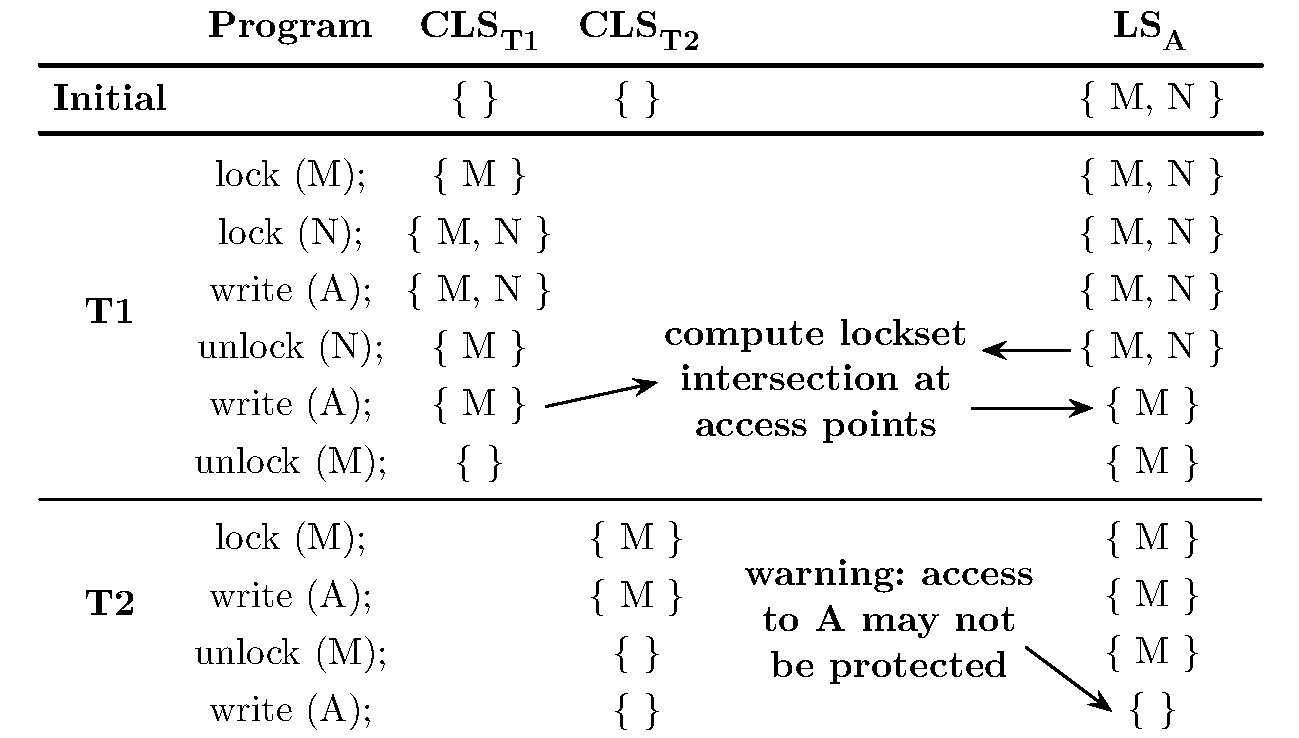
\includegraphics[width=1\linewidth]{img/lockset.pdf}
%\vspace{-5mm}
\caption{Applying lockset analysis on a concurrent program.}
\label{fig:locksets}
%\vspace{-3mm}
\end{figure}


\section{The \whoop Approach}
\label{whoop}


We now present \emph{symbolic pairwise lockset analysis}, a novel method for data race analysis in device drivers.  In \S\ref{sec:symbolicpairwise} we describe how the approach works in a semi-formal manner, with respect to a simple concurrent programming model.  In \S\ref{sec:implementation} we explain how we have implemented symbolic pairwise lockset analysis in a practical tool, \whoop, that can be applied directly to driver source code.

Our experimental evaluation (\S\ref{evaluation}) demonstrates that the \whoop technique has value as a stand-alone analyzer, and that results from \whoop can be exploited to significantly boost the performance of a more precise symbolic analysis for concurrency, based on context bounding and stratified inlining, offered by the \corral~\cite{lal2012corral} tool; we discuss the latter approach in \S\ref{corral}.

\subsection{Symbolic Pairwise Lockset Analysis}
\label{sec:symbolicpairwise}

Our approach considers, for a given driver, every pair of entry points that can potentially execute concurrently.  For each such pair, we use symbolic verification to check whether it is possible for the pair to race on a shared memory location. We soundly model the effects of additional entry points by treating the driver shared state abstractly: when an entry point reads from the shared state, a nondeterministic value is returned.  Restricting to pairs of entry points, rather than analysing all entry points simultaneously, exploits the fact that data races occur between pairs of threads and allows our analysis to scale to large drivers.  The trade-off is that a quadratic number of entry point pairs must be checked.  In \S\ref{sec:implementation} we discuss optimizations based on device driver domain knowledge to reduce the number of pairs to some extent.

Symbolic verification of a pair of entry points works by (i) instrumenting each entry point with additional state to record locksets, and (ii) attempting to verify a sequential program that executes the instrumented entry points in sequence and then asserts, for each shared location, that the locksets for each entry point with respect to this location have a non-empty intersection.  Verification of the resulting sequential program can be undertaken using any sound method; in practice we employ the Boogie verification engine~\cite{barnett2006boogie}, which requires procedure specifications and loop invariants to be generated, after which verification conditions~\cite{barnett2005weakest} (VCs) are generated and discharged to an automated theorem prover.

We now detail the approach in a semi-formal manner, in the context of a simple concurrent programming model.

\medskip\noindent\textbf{Concurrent Programming Model }
%
We consider a concurrent programming model where an unbounded number of threads execute a set of pre-defined \emph{thread templates}.  At any given point of execution a certain number of threads are active, each thread executing a particular template.  In the context of device drivers, a thread template corresponds to a driver entry point, and multiple instances of the same thread template may execute concurrently, just as multiple invocations of a single driver entry point may be concurrent.  Further threads may be launched at any point during execution; in the context of device drivers this corresponds to the OS invoking additional driver entry points.  For ease of presentation only, our model does not feature aggregate data types, pointers or dynamic memory allocation.  These \emph{are} handled by our implementation, and in \S\ref{sec:implementation} we discuss interesting practical issues arising from the handling of a full-blown language.

A \emph{concurrent program} is described by a finite set of \emph{shared} variables, $\sharedvars$, a finite set of mutexes, $\mutexes$, and a finite set of \emph{thread templates}.  A thread template, $T$, consists of a finite set of procedures, $\procedures{T}$, and a finite set of private variables, $\variables{T}$.  A designated procedure, $\mainforthread{T} \in \procedures{T}$, denotes the starting point for execution of $T$ by a thread.  Each procedure of $\procedures{T}$ is represented by a control flow graph of basic blocks, where each block contains a sequence of statements.  A basic block either has a single successor or a pair of successors.  In the latter case, an \emph{exit condition} over thread-private variables determines the successor to which control should flow on block exit.

The forms of statements are shown in Figure~\ref{fig:statements}, and include designated statements for reading from and writing to shared variables.  In particular, shared variables may not appear in arbitrary expressions.  This restriction simplifies our presentation of lockset instrumentation, below, and a program that does not satisfy this restriction can be trivially pre-processed into one that does via the introduction of additional private temporary variables to record values read from the shared state.  We do not specify the form of expressions, nor the types of variables, assuming a standard set of data types and operations.

\begin{figure}
\begin{tabular}{lp{5.5cm}}
\textbf{Statement Form} & \textbf{Notes} \\
\toprule

$x = e;$ & private assignment, where $x \in \variables{T}$ and $e$ is an expression over $\variables{T}$ \\
\midrule

$x = f(\overline{e});$ & procedure call, where $x \in \variables{T}$, $\overline{e}$ is a sequence of expressions over $\variables{T}$, $f$ is the name of a procedure in $\procedures{T}$ \\
\midrule

$s = e;$ & shared write, where $s \in \sharedvars$ and $e$ is an expression over $\variables{T}$ \\
\midrule

$x = s;$ & shared read,  where $x \in \variables{T}$ and $s \in \sharedvars$ \\
\midrule

$\mutexlock{m};$   & mutex lock, where $m \in \mutexes$ \\
\midrule

$\mutexunlock{m};$ & mutex unlock, where $m \in \mutexes$\\
\bottomrule
\end{tabular}
\caption{Forms of statements in our simple programming model}
\label{fig:statements}
\end{figure}

\medskip\noindent\textbf{Semantics }
%
Let $\ids$ be an infinite set from which dynamic thread ids will be drawn.  The state of a running concurrent program consists of: a valuation of the shared variables, $\sharedvars$; a mapping that associates each mutex in $\mutexes$ with an id from $\ids$, recording which thread currently holds the mutex, or with a special value $\bot \notin \ids$ to indicate that the mutex is not held by any thread; and a list of \emph{threads}.  Each thread consists of an id, drawn from $\ids$, a thread template, $T$, an index indicating the next statement of $T$ to be executed by the thread, and a valuation of the thread private variables, $\variables{T}$.  If multiple threads are instances of the same template $T$, then each thread carries a \emph{separate} valuation of the private variables for this template.

At the start of execution the valuation of shared variables is arbitrary, no mutexes are held (i.e.\ each mutex maps to $\bot$), and the list of threads is empty.
%
At any point of execution, a new thread may be added to the list of threads.  This involves selecting a thread template $T$ and an id $i \in \ids$ that has not been previously used during program execution, setting the point of execution for the new thread to be the first statement of $\mainforthread{T}$, and choosing an arbitrary valuation for the private variables $\variables{T}$.

We consider a standard interleaving model of concurrency: at any execution point, a thread may execute its current statement, unless that statement has the form $\mutexlock{m}$ and mutex $m$ is already held by some thread.  Executing a statement causes the state of the thread, and the shared state, to be updated in a standard manner.  For example, if a thread following template $T$ executes $s = e$, where $s \in \sharedvars$ and $e$ is an expression over $\variables{T}$, the shared variable valuation is updated so that $s$ has the value determined by evaluating $e$ in the context of the thread's private variable valuation.  Because our interest is in data race analysis for race-free programming, we are not concerned with relaxed memory behavior: race-free programs exhibit only sequentially consistent behaviors.

A thread terminates if it reaches the end of $\mainforthread{T}$; in this case the thread is removed from the list of threads.  Because we are interested in the analysis of device drivers, which are \emph{reactive} concurrent programs, we do not consider the notion of global program termination.

\medskip\noindent\textbf{Lockset Instrumentation }
%
For thread templates $T$ and $U$ (including the possibility that $T$ and $U$ are equal) we wish to check whether it is possible for a thread executing $T$ to race with a thread executing $U$, in the presence of arbitrarily many further concurrently executing threads.

To achieve this, we first \emph{instrument} a thread template for lockset analysis (see \S\ref{bg:lockset}).  Given an arbitrary symbol, $i$, we define the instrumentation of a template $T$ with respect to $i$, denoted $\instrument{T}{i}$.  There are two aspects to this instrumentation phase: \emph{renaming} and \emph{lockset instrumentation}.

Renaming is straightforward: all occurrences of private variable $x \in \variables{T}$ used in $T$ are replaced with a renamed variable $\instrument{x}{i}$ in $\instrument{T}{i}$, and every procedure $f \in \procedures{T}$ is renamed (both at its declaration site and at all call sites) to $\instrument{f}{i}$ in $\instrument{T}{i}$.  The purpose of renaming is to ensure that when we analyze a pair of templates, $T$ and $U$, both templates execute distinct procedures and operate on distinct private data.  This is vital in the case where $T$ and $U$ are the same.

\begin{figure}
\begin{tabular}{ll}
\textbf{Original Statement} & \textbf{Instrumented Statement} \\
\toprule

$s = e;$ & $\hasbeenwritten{i} = \hasbeenwritten{i} \cup \{ s \};$ \\
         & $\lockset{s}{i} = \lockset{s}{i} \cap \currentlockset{i};$ \\
\midrule
         
$x = s;$ & $\hasbeenread{i} = \hasbeenread{i} \cup \{ s \};$ \\
         & $\lockset{s}{i} = \lockset{s}{i} \cap \currentlockset{i};$ \\
         & $\havoc{\instrument{x}{i}};$ \\
\midrule
         
$\mutexlock{m};$   & $\currentlockset{i} = \currentlockset{i} \cup \{ m \};$ \\
\midrule

$\mutexunlock{m};$ & $\currentlockset{i} = \currentlockset{i} \setminus \{ m \};$ \\
\bottomrule
\end{tabular}
\caption{Instrumenting statements for lockset analysis}
\label{fig:instrumentation}
\end{figure}

Lockset instrumentation introduces: sets $\hasbeenread{i} \subseteq \powerset{\sharedvars}$ and $\hasbeenwritten{i} \subseteq \powerset{\sharedvars}$ to track the shared variables that have been read from and written to, respectively, by the thread executing $T$; a current lockset, $\currentlockset{i} \subseteq \powerset{\mutexes}$, to record the mutexes that are currently held by the thread; and, for each shared variable $s \in \sharedvars$, a lockset, $\lockset{s}{i}$, to record the mutexes that are consistently held when the thread accesses $s$.

The statements of each procedure in $\instrument{T}{i}$ that access shared variables and mutexes are instrumented to manipulate these sets.  This transformation is described in Figure~\ref{fig:instrumentation}, where for an expression $e$ we use $\instrument{e}{i}$ to denote $e$ after renaming with respect to $i$.  A shared variable assignment, $s = e$, is instrumented by recording in $\hasbeenwritten{i}$ that $s$ has been written to, and updating the lockset for $s$, $\lockset{s}{i}$, to eliminate any mutexes that are not currently held (i.e.\ those mutexes that are not in $\currentlockset{i}$).  A shared variable read, $x = s$ operates analogously, except for the additional $\havockeyword$ command which we discuss under \emph{Shared State Abstraction} below.  Instrumentation of mutex manipulation commands, $\mutexlock{m}$ and $\mutexunlock{m}$, involves updating the current lockset, $\currentlockset{i}$, to add and remove mutex $m$, respectively.

\medskip\noindent\textbf{Shared State Abstraction }
%
Recall that while our aim is to perform race analysis for pairs of threads, we must be sure to account for possible side-effects due to other threads that are running concurrently.  The instrumentation of Figure~\ref{fig:instrumentation} achieves this via \emph{nondeterminism}: when reading from a shared variable $s$, a nondeterministic value is returned.  This is reflected by the use of a $\havockeyword$ command, which sets its argument to an arbitrary value.  Because all shared state accesses are abstracted in this fashion, it is possible to completely dispense with the shared variables after the lockset instrumentation has been performed.  As a result, when instrumenting a shared variable write, the effect of the write is not explicitly modeled.

\medskip\noindent\textbf{Sequentialisation }
%
The pseudocode of Figure~\ref{fig:sequentialization} shows the sequential program that we analyze in order to prove race-freedom for a pair of thread templates $T$ and $U$. Assuming that $T$ and $U$ have been instrumented using distinct symbols $i$ and $j$, yielding $\instrument{T}{i}$ and $\instrument{U}{j}$, the sequential program operates as follows. First, the read, write and current locksets for $\instrument{T}{i}$ and $\instrument{U}{j}$ are initialized to be empty, and for each shared variable $s$, the locksets $\lockset{s}{i}$ and $\lockset{s}{j}$ are initialized to the full set of mutexes, $\mutexes$.  The main procedures of the instrumented thread templates, $\mainforthread{\instrument{T}{i}}$ and $\mainforthread{\instrument{U}{j}}$, are then executed in turn (the order does not matter, due to renaming). Finally, an assertion checks for consistent use of mutexes: if $s$ is written during execution of $\instrument{T}{i}$ and accessed during execution of $\instrument{U}{j}$, or vice-versa, then the locksets $\lockset{s}{i}$ and $\lockset{s}{j}$ must contain at least one common mutex.

\begin{figure}
\begin{tabular}{l}
$\currentlockset{i} = \emptyset;$ $\hasbeenread{i} = \emptyset;$ $\hasbeenwritten{i} = \emptyset;$ \\
$\currentlockset{j} = \emptyset;$ $\hasbeenread{j} = \emptyset;$ $\hasbeenwritten{j} = \emptyset;$ \\
\texttt{for} $s \in \sharedvars$ \texttt{do} $\lockset{s}{i} = \mutexes;$ $\lockset{s}{j} = \mutexes;$ \medskip
\\

$\mainforthread{\instrument{T}{i}}();$ \\
$\mainforthread{\instrument{U}{j}}();$ \medskip\\

\texttt{assert} $\forall s \in \sharedvars \; .$ \\

$\quad s \in \hasbeenwritten{i} \cap (\hasbeenread{j} \cup \hasbeenwritten{j}) \vee s \in \hasbeenwritten{j} \cap (\hasbeenread{i} \cup \hasbeenwritten{i}) \implies$ \\

$\quad\quad \lockset{s}{i} \cap \lockset{s}{j} \neq \emptyset;$ \\

\end{tabular}
\caption{The sequential program to be analyzed in order to prove race-freedom for a pair of thread templates}
\label{fig:sequentialization}
\end{figure}

\medskip\noindent\textbf{Soundness }
%
We sketch an argument that if the program of Figure~\ref{fig:sequentialization} is correct, it is impossible for a thread executing template $T$ to race with a thread executing template $U$, under the assumption that the threads are guaranteed to terminate. Let us assume that the program of Figure~\ref{fig:sequentialization} is correct, and suppose (by way of contradiction) that a thread executing $T$ can in fact race with a thread executing $U$, on some shared variable $s$.  By our hypothesis that the program of Figure~\ref{fig:sequentialization} is correct, and that the threads terminate, the assertion checked at the end of the program guarantees at least one mutex, say $m$, belongs to both $\lockset{s}{i}$ and $\lockset{s}{j}$.  By the definition of a lockset (and according to the manner in which shared accesses are instrumented in Figure~\ref{fig:instrumentation}), this means that $m$ is held during every access to $s$ by both $\instrument{T}{i}$ and $\instrument{U}{j}$. As a result, $m$ must be unlocked and locked between the two accesses, which contradicts that the pair of accesses is racing.

We require the threads to terminate because in the presence of non-termination the assertion at the end of Figure~\ref{fig:sequentialization} may not be reached.  The termination analysis problem for device drivers has been widely studied, notably in the context of the Terminator tool~\cite{cook2006termination}. In the remainder of the paper we do not consider termination issues, assuming that the drivers we analyze in our experimental evaluation (see \S\ref{evaluation}) are indeed terminating.

\subsection{Implementation in \whoop}
\label{sec:implementation}

The simple concurrent programming model of \S\ref{sec:symbolicpairwise} is deliberately idealistic to make it easy to describe our symbolic verification technique. In practice, Linux drivers are written in C, we do not know up-front which are the entry points for a driver, drivers do not work with a cleanly specified set of named locks, and rather than having a given set of named shared variables, we have arbitrary memory accesses via pointers. We now explain how we have taken the conceptual ideas from \S\ref{sec:symbolicpairwise} and used them to build \whoop, a practical, fully automatic tool for detecting data races in drivers.

\begin{figure*}
\centering
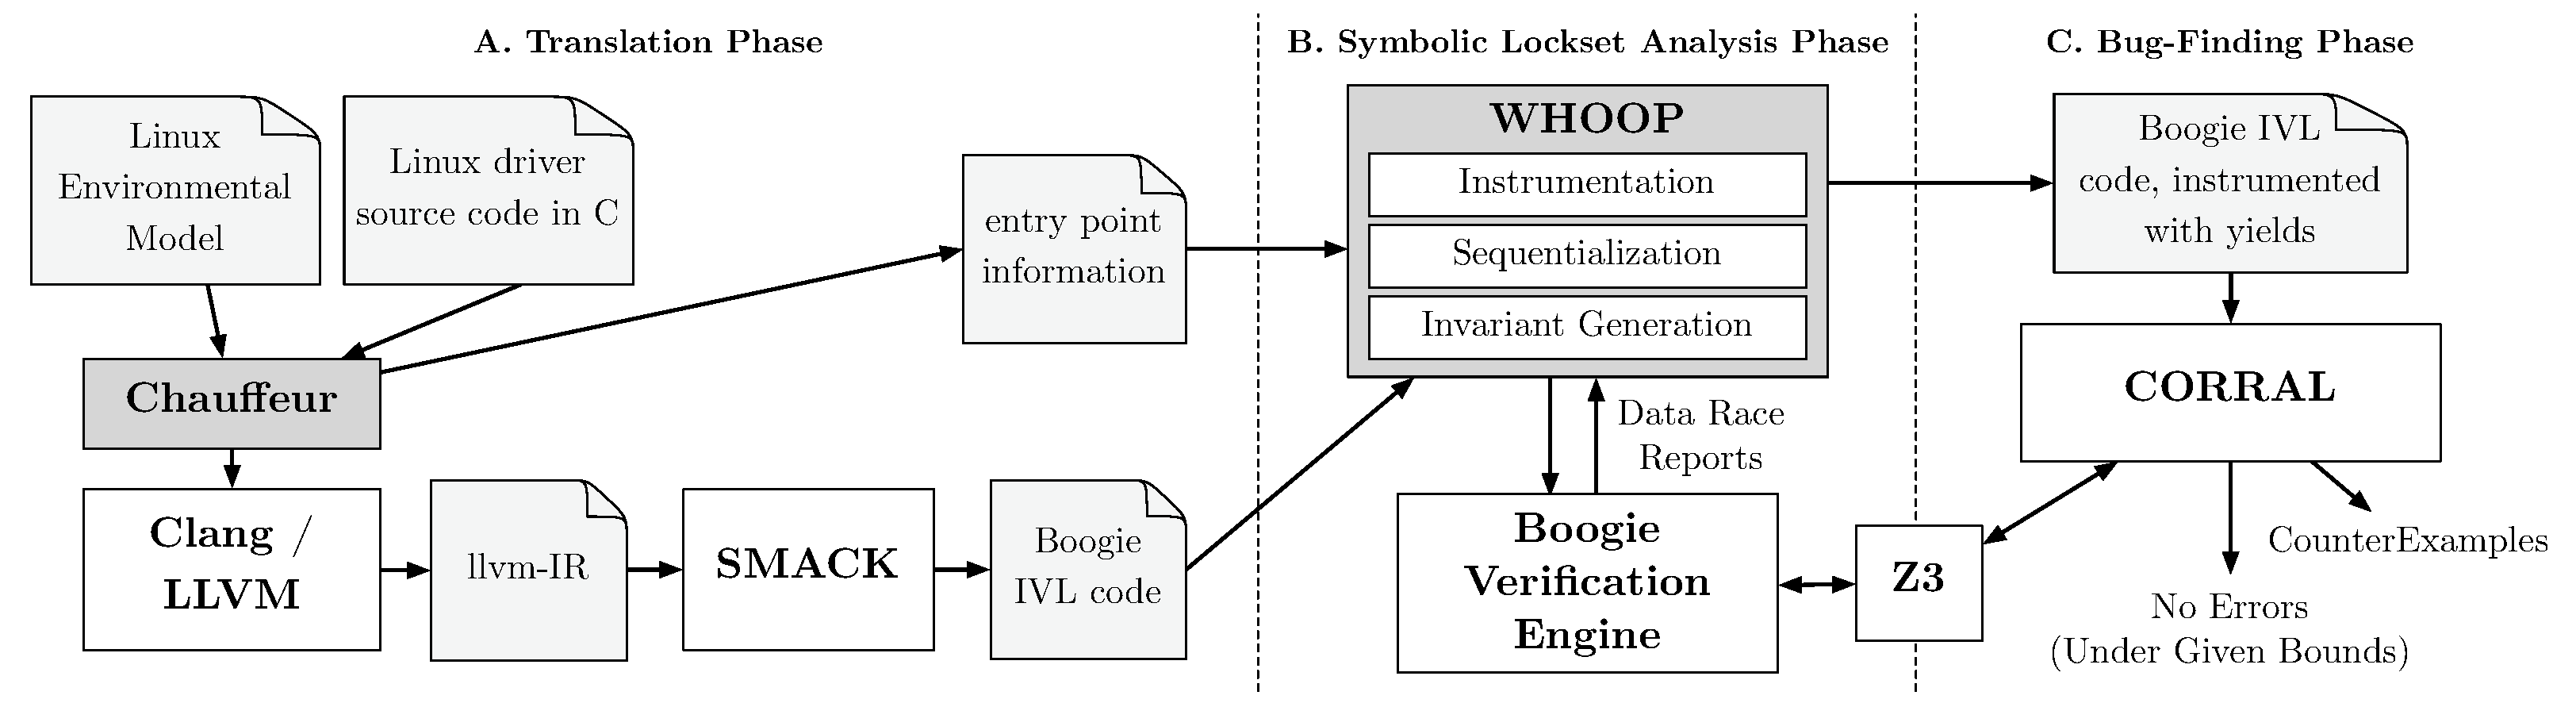
\includegraphics[width=.99\linewidth]{img/whoop.pdf}
\caption{The \whoop architecture, empowered by state-of-the-art compilation (Clang/LLVM and SMACK) and verification (Boogie and \corral) tools}
\label{fig:whoop}
\end{figure*}

\medskip\noindent\textbf{Architecture }
%
Figure~\ref{fig:whoop} depicts the \whoop toolchain. Initially, \whoop accepts a Linux driver written in C, together with an environmental model\footnote{This consists of stub header files modeling relevant Linux kernel APIs.} that is required to ``close'' the driver and allow it to be subsequently analyzed for data races. Both the driver and the Linux model are passed to the translation phase of \whoop (see Figure~\ref{fig:whoop} -- A), which uses three LLVM\footnote{\url{http://llvm.org}}-based tools, Chauffeur\footnote{\url{https://github.com/mc-imperial/chauffeur}}, Clang\footnote{\url{http://clang.llvm.org}} and SMACK\footnote{\url{https://github.com/smackers/smack}}~\cite{rakamaric2014smack}, to translate the original driver into an abstract program written in the Boogie intermediate verification language (IVL)~\cite{deline2005boogiepl}, a simple imperative language with well-defined semantics that is used as the input to a number of cutting-edge verifiers (e.g.\ Boogie and \corral).

Next, \whoop instruments and sequentializes the program to perform symbolic pairwise lockset analysis (see Figure~\ref{fig:whoop} -- B and \S\ref{sec:symbolicpairwise}) using the Boogie verification engine. After the verification phase ends, \whoop can exploit any inferred race-freedom guarantees to accelerate precise race-checking with \corral (see Figure~\ref{fig:whoop} -- C and \S\ref{corral}).

We engineered the Chauffeur and \whoop components of our toolchain (denoted with grey boxes in Figure~\ref{fig:whoop}).  For the remaining components, we were able to re-use industrial-strength tools that are robust and battle-proven via their use in many complex software projects.

\medskip\noindent\textbf{Extracting Entry Point Information }
%
Chauffeur is a Clang-based frontend that traverses the abstract syntax tree (AST) of the original driver (using a Clang visitor pass) and extracts all entry point identifier names, together with the identifier names of their corresponding kernel API functions. Linux drivers define entry points in a standard way (see Figure~\ref{fig:entrypoints} for an example of how the generic\_nvram driver defines the entry points for the \texttt{file\_operations} API); Chauffeur identifies these definitions in the AST and outputs the relevant information in an XML file, which is subsequently parsed by \whoop and used during the instrumentation.

\begin{figure}[t]
\begin{lstlisting}
const struct file_operations nvram_fops = {
  .llseek = nvram_llseek,
  .read = read_nvram,
  .write = write_nvram,
  .unlocked_ioctl = nvram_unlocked_ioctl,
};
\end{lstlisting}
\caption{Entry points definitions in the generic\_nvram driver}
\label{fig:entrypoints}
\end{figure}

\medskip\noindent\textbf{Translation for Verification }
%
Next, the driver is compiled by Clang to LLVM-IR~\cite{lattner2004llvm}, a low-level assembly-like language in single static assignment (SSA) form. Function calls (e.g.\ for locking and unlocking) are preserved in this translation, which is useful for our lockset instrumentation.

SMACK then translates the driver from LLVM-IR to Boogie IVL, which is the input language of \whoop. An important feature of SMACK is that it leverages the pointer-alias analyses of LLVM to efficiently model the heap manipulation operations of C programs in Boogie IVL. This means that \whoop does not need to directly deal with pointers and alias analysis, a hard problem on its own, allowing us to re-use robust existing techniques and focus instead on verification efforts.

To achieve scalability, SMACK uses a \emph{split} memory model that exploits the case where
alias analysis asserts that a given memory location cannot be aliased by multiple types.
This has been shown to lead to more tractable verification compared with a \emph{monolithic} model where the heap is considered to be an array of bytes~\cite{rakamaric2009scalable}. This split memory model is based on \emph{memory regions}, which are maps of integers that model the heap. A benefit of using this model is that distinct memory regions denote disjoint sections of the heap. We leverage this knowledge inside \whoop to guide and optimize our lockset instrumentation and analysis, and to create a fine-grained context-switch instrumentation as discussed in \S\ref{corral}.

\medskip\noindent\textbf{Identifying Locks }
%
When the instrumentation phase begins, \whoop performs an inter-procedural static analysis (on the Boogie IVL source code of each entry point) to identify all available locks and rewrite each one (both at declaration and at all access sites) to a unique constant Boogie variable. The reason behind this transformation, is that representing all locks statically, instead of their original SMACK pointer-based representation, helps \whoop perform various internal instrumentation and optimization passes.
%
Currently, \whoop only supports mutexes and spinlocks that are available in the Linux kernel APIs. However, it is relatively easy to enhance our tool with knowledge of other locking primitives. If \whoop cannot infer a lock, e.g. because it was created dynamically or was indexed from an array of locks, it will exit with a warning. The are two reasons behind this: (i) it is arguably hard to detect such locks using static analysis; and (ii) a small, fixed number of locks is advocated by Linux experts as good practice when developing drivers~\cite{corbet2005linux}.

\medskip\noindent\textbf{Watchdog Race-Checking Instrumentation }
%
Data race detection is performed by introducing sets containing the locks that are consistently held by each shared variable and sets containing all shared variables that are read and written (see \S\ref{sec:symbolicpairwise} and the instrumentation of Figure~\ref{fig:instrumentation}). These sets can be modeled directly in Boogie as characteristic functions, using maps. However, this requires the use of quantifiers to express properties related to set contents.  For instance, to express that a set $X$ of elements of type $A$ is empty, where $X$ is represented as a map from $A$ to $\mathsf{Bool}$, we would require the quantified expression $\forall a : A : \neg X[a]$.  It is well known that automated theorem proving in the presence of quantified constraints is challenging, and that theorem provers such as Z3~\cite{de2008z3} are often much more effective when quantifiers are avoided.  

To avoid quantifiers and the associated theorem proving burden, we use instead a \emph{watchdog race-checking instrumentation}, adapted from~\cite{bardsley2014engineering}.  Suppose we are analysing entry points $T$ and $U$, and that after translation into Boogie these entry points share a common memory region, $\mathit{MR}$.  When analyzing $T$ and $U$ for races, we introduce an unconstrained symbolic constant $\mathit{watched}_{\mathit{MR}}$, representing some unspecified index into $\mathit{MR}$; we call this the \emph{watched offset} for $\mathit{MR}$.  We then attempt to prove that it is impossible for $T$ and $U$ to race on $\mathit{MR}$ at index $\mathit{watched}_{\mathit{MR}}$.  If we can succeed in proving this, we know that $T$ and $U$ must be race-free for the \emph{whole} of $\mathit{MR}$, since the watched offset was arbitrary.  This technique of choosing an arbitrary index to analyse for each map manipulated by an entry point pair can be seen as a form of quantifier elimination: rather than asking the underlying theorem prover to reason for all indices of $\mathit{MR}$, in a quantified manner, we eliminate the quantifier in our encoding, and instead ask the theorem prover to reason about a single, but arbitrary, index of $\mathit{MR}$.

\medskip\noindent\textbf{Watchdog Summarization }  \ADComment{Due to my thoughts below, I'm unsure about calling this ``Watchdog'' summarization, as I don't think we're doing anything new here.  I think perhaps ``Generatino of Loop and Procedure Summaries'' would be better.}
%
Early in the development of \whoop we experimented with reasoning about recursion-free drivers by resorting to full inlining.  We found that this did not scale to large drivers: when we tried to apply \whoop to the r8169 ethernet driver ($>$7000 lines of C code) with all functions fully inlined, we quickly exhausted the memory limits of our experimental platform.  \ADComment{Is it thus the case that r8169 did not exhibit any recursion?}  The C-to-Boogie translation produced, after inlining, hundreds of thousands of lines of Boogie IVL code, consuming a lot of memory and leading to gigantic verification conditions that the Z3 theorem prover could not handle effectively.  \ADComment{I rephrased the previous sentence, because if I remember correctly we did get to the point of invoking Z3.  But maybe I imagined that - perhaps we could not even generate the VC?}  Furthermore, some entry points invoke recursive helper functions, which cannot be fully inlined.

\ADComment{I think the following is the weakest part of this (in general very good) section at the moment.  My concerns are that (a) we have not really invented anything new, we just applied Houdini having guessed candidate preconditions, postconditions and loop invariants based on heuristics, and (b) we have not given much intuition for what these candidates look like.  Could you give an example candidate, using mathematical notation?  For instance, if entry point $T$ has a procedure $f$ that releases mutex $m$, then when instrumenting $T$ with symbol $i$ (using the notation from \S\ref{sec:symbolicpairwise}) we might guess $m \notin \currentlockset{i}$ as a postcondition for $\instrument{f}{i}$.  It would be ideal if you could be as specific as possible about the candidates we generate.}

To make our analysis scalable, and to cater for recursion, we developed \emph{watchdog summarization}, a novel summarization technique that allows us to analyze drivers in a scalable fashion and without destroying precision.
Watchdog summarization uses the Houdini~\cite{flanagan2001houdini} invariant inference algorithm (available inside Boogie) to automatically compute summaries (pre- and post-conditions and loop invariants) from a pool of \emph{candidate} invariants.  The Boogie verifier then automatically checks whether each procedure meets its summary, abstracting each called procedure with its summary in the process; Boogie also checks whether loops respect their invariants and uses the invariants to over-approximate the effects of loops.

The candidate invariants are based on the aforementioned global watchdog variables that \whoop instruments for watchdog race-checking. The key idea behind watchdog summarization is to automatically generate candidate invariants for each memory region in the granularity of watched accesses. This reduces the false positives from reporting errors if only e.g.\ a field in memory region $\mathit{MR}$ is racing, but the rest of the fields in $\mathit{MR}$ are not racing.

To generate the candidate invariants, \whoop performs an inter-procedural static analysis on the call-graph (in Boogie IVL code) of each entry point, identifying all possible accesses to shared memory locations. To be sound, if \whoop cannot infer information for a specific access, it generates a coarse-grained candidate for the corresponding memory region.

\ADComment{In the above, can you make it super-clear that it is fine for the candidates to be wrong: Houdini will just kick them out?  You might want to look at the comment on this in the GPUVerify 2012 OOPSLA paper; I remember writing something nice along these lines, feel free to re-use it.  If you search for Houdini you'll find it.}

\medskip\noindent\textbf{Verification and Error Reporting }
%
For each pair of entry points, the instrumented sequential program, equipped with procedure and loop summaries, is sent to the Boogie verification engine. Boogie generates a VC, for each procedure in the program, and discharges it to the Z3~\cite{de2008z3} theorem prover.  In particular, the verification for the root-level procedure, encoding the sequential program sketched in Figure~\ref{fig:sequentialization}, encodes the race-freedom check for the entry point pair. Successful verification implies that the entry point pair is free of data races, while an error (i.e.\ counterexample) denotes a \emph{potential} data race and is reported to the user. To improve usability, \whoop has a built-in error reporter that matches counterexamples to source code. The following is a race that \whoop found and reported for the example of Figure~\ref{fig:data_race_example}: 

\begin{lstlisting}[keywordstyle=\ttfamily]
generic_nvram.c: error: potential read-write race:
  read by entry point nvram_llseek, generic_nvram.c:54:2
    return file->f_pos;
  write by entry point nvram_llseek, generic_nvram.c:53:2
    file->f_pos = offset;
\end{lstlisting}

Because a driver is processed by Clang and SMACK during the translation from C to Boogie IVL, significant engineering effort was required to map Boogie-level errors back to original source code locations.

\medskip\noindent\textbf{Optimizations }
%
We have implemented various optimizations to increase the precision and performance of \whoop.  We comment on the two most effective optimizations.

First, we enriched \whoop with information regarding \emph{kernel-imposed serialization}, to increase precision. The Linux kernel can serialize calls to entry points, thus forcing them to run sequentially with each other. As an example, a large number of networking entry points are mutually serialized with RTNL, a network-specific kernel lock. We discovered this when we first analyzed the r8169 driver (see \S\ref{evaluation}) and \whoop reported many races between a number of networking entry points; when we investigated the source of these races, we found out that these entry points could not race in reality because of RTNL. \whoop exploits this knowledge and does not create pairs for entry points that are serialized by the kernel. This is an ongoing manual effort: the more drivers we study, the more such properties we discover, which we can then exploit to make \whoop more precise. Currently, this information is hard-coded inside \whoop. In the future, we plan to provide a configuration file where the user can denote such kernel specific information.

Second, we soundly reduce the number of memory regions that are analyzed for races.  If memory region $\mathit{MR}$ is accessed by only one entry point in a pair then, trivially, the pair cannot race on $\mathit{MR}$.  We thus disable lockset analysis for $\mathit{MR}$.  This can reduce the complexity of VCs that need to be solved by the theorem prover, speeding up the verification process.

\medskip\noindent\textbf{Practical Assumptions Related to Soundness}
%
\whoop is ``soundy''\footnote{http://soundiness.org/}~\cite{soundiness}: it aims in principle to perform a sound analysis that can prove absence of races, but suffers from some known sources of unsoundness, which we now comment on.

We assume that the formal parameters of an entry point do not alias, and thus cannot race. This is a potentially unsound feature that can be turned off using a command line option, but without this assumption the false alarm rate of \whoop is very high. In our experience so far, we have not missed any races by assuming non-overlapping parameters.  We also rely on the soundness of our best-effort environmental model, and on exploiting domain-specific knowledge related to entry point serialization by the Linux kernel.

As well as inheriting soundness issues arising from currently unknown bugs in \whoop and in the external tools that \whoop relies on, we acknowledge that SMACK is subject to sources of unsoundness (e.g.\ SMACK models integers as an infinite set, rather than as a finite set of bit-vectors) and that the combination of Clang and SMACK commits our approach to specific choices related to undefined and implementation-defined aspects of the C language when translating to Boogie.  However, \whoop makes no fundamental assumptions related to these translation decisions, meaning that a more accurate C-to-Boogie translation would automatically lead to a more accurate analysis with \whoop.

\medskip\noindent\textbf{Limitations }
%
\whoop is based on lockset analysis and thus can report false bugs, because a violation of the locking discipline does not always correspond to a real data race (e.g.\ when lockfree synchronization is used instead of locking). \whoop also uses over-approximation (e.g.\ when reading from the shared state) and summarization, which can be sources of false positives. Furthermore, the tool does not currently check for dynamically created locks or for locks that are provided by external libraries, although the later could be addressed by providing a mechanism for users to declare custom locks. We also do not currently handle interrupt handlers in a special way; to be sound, we assume that they can execute concurrently with entry points at any time. We could address this in the future by modeling interrupt-specific kernel functions (e.g. for enabling/disabling interrupts).

Another limitation of \whoop is that it is unable to verify drivers that are designed to be accessed by a single process at a time. This \emph{single-open device}~\cite{corbet2005linux} mode can be enforced by atomically testing (at the beginning of each entry point) a flag that indicates device availability: if the flag is set to true, then the respective entry point executes, else it blocks. Because \whoop performs pair-wise analysis, it over-approximates this flag, and regards a pair of entry points as running concurrently, even if this is not the case. However,~\cite{corbet2005linux} advises against serializing drivers in this way, as it hinders user ingenuity (e.g.\ a user might expect that a device can be accessed concurrently for performance). Because using single-open device mode is considered bad practice, we thus burden the developer with disregarding any related false bug reports.

Statically analyzing system-level software, such as drivers, requires to ``close'' the environment by abstracting away the low level implementation details. In this work, we developed a simple environmental model for the Linux kernel that consists of (nondeterministic) stub functions. A limitation of our model is that it can, and will, ultimately result in decreased precision and, thus, false positives. However, because we currently only focus on finding data races, we can get away with over-approximating a lot of the underlying Linux kernel functionality, without losing too much precision. Enriching our model with domain-specific knowledge to make it more precise is an ongoing manual effort, but requires Linux expertise. We argue that further increasing the precision is orthogonal to the contributions of this paper. Moreover, even if the symbolic lockset analysis results in false positives, \whoop can still use any race-freedom guarantees to significantly speedup a more precise bug-finder, as seen in \S\ref{corral} and \S\ref{evaluation}.


\section{Evaluation}
\label{evaluation}

\newcommand{\colspacing}{\hspace{1.8em}}
\begin{table}[t]
\small
\centering
\setlength{\tabcolsep}{0.3em}
\caption{Program statistics and race-checking results from applying \whoop and \corral on our benchmarks.}
\label{tab:stats}
\begin{tabular}{l rrr rr r}
\centering
& & & & \multicolumn{2}{c}{\textbf{\whoop}}
& \textbf{\corral}\\
\cmidrule(lr){5-6}
\cmidrule(lr){7-7}

& & & & \multicolumn{1}{r}{\textbf{\#Racy}}
& \multicolumn{1}{r}{\textbf{\#Racy}}
& \multicolumn{1}{r}{\textbf{\#Races}}\\

\textbf{Benchmarks}
& \textbf{LoC}
& \textbf{\#Pairs}
& \textbf{\#MRs}
& \multicolumn{1}{r}{\textbf{Pairs}}
& \multicolumn{1}{r}{\textbf{MRs}}
& \multicolumn{1}{r}{\textbf{Found}}\\[0.3em]

\toprule

generic\_nvram
& 283
& 14
& 39
& \multicolumn{1}{r}{7}
& \multicolumn{1}{r}{2}
& 4\\

pc8736x\_gpio
& 354
& 27
& 55
& \multicolumn{1}{r}{13}
& \multicolumn{1}{r}{6}
& 5\\

machzwd
& 457
& 10
& 49
& \multicolumn{1}{r}{6}
& \multicolumn{1}{r}{3}
& 1\\

ssu100
& 568
& 7
& 27
& \multicolumn{1}{r}{\xmark}
& \multicolumn{1}{r}{\xmark}
& \xmark\\

intel\_scu\_wd
& 632
& 10
& 45
& \multicolumn{1}{r}{5}
& \multicolumn{1}{r}{1}
& 2\\

ds1286
& 635
& 15
& 49
& \multicolumn{1}{r}{5}
& \multicolumn{1}{r}{3}
& \xmark\\

dtlk
& 750
& 21
& 53
& \multicolumn{1}{r}{10}
& \multicolumn{1}{r}{6}
& \xmark\\

fs3270
& 883
& 15
& 54
& \multicolumn{1}{r}{9}
& \multicolumn{1}{r}{1}
& \xmark\\

gdrom
& 890
& 94
& 41
& \multicolumn{1}{r}{21}
& \multicolumn{1}{r}{2}
& \xmark\\

swim
& 996
& 28
& 80
& \multicolumn{1}{r}{15}
& \multicolumn{1}{r}{7}
& 8\\

intel\_nfcsim
& 1272
& 10
& 24
& \multicolumn{1}{r}{10}
& \multicolumn{1}{r}{2}
& \xmark\\

ps3vram
& 1499
& 4
& 32
& \multicolumn{1}{r}{1}
& \multicolumn{1}{r}{1}
& \xmark\\

sonypi
& 1729
& 30
& 62
& \multicolumn{1}{r}{19}
& \multicolumn{1}{r}{4}
& 2\\

sx8
& 1751
& 2
& 47
& \multicolumn{1}{r}{2}
& \multicolumn{1}{r}{1}
& 1\\

8139too
& 2694
& 46
& 37
& \multicolumn{1}{r}{40}
& \multicolumn{1}{r}{4}
& \xmark\\

r8169
& 7205
& 192
& 50
& \multicolumn{1}{r}{88}
& \multicolumn{1}{r}{1}
& \xmark\\

\bottomrule
\end{tabular}
\end{table}

\begin{table*}[t]
\small
\centering
\setlength{\tabcolsep}{0.45em}
\caption{Comparison with different yield instrumentation granularities and context-switch bounds.}
\label{tab:results}
\begin{tabular}{l r rrrr rrrr rrrr}
\centering
& \textbf{\whoop}
& \multicolumn{3}{c}{\textbf{\corral}}
& \multicolumn{6}{c}{\textbf{\whoop + \corral}}\\
\cmidrule(lr){2-2}
\cmidrule(lr){3-5}
\cmidrule(lr){6-11}

& \multirow{2}{*}{\textbf{Time}}
& \multicolumn{3}{c}{\textbf{\yieldall\xspace --- Time (sec)}}
& \multicolumn{3}{c}{\textbf{\yieldcoarse\xspace --- Time (sec)}}
& \multicolumn{3}{c}{\textbf{\yieldmr\xspace --- Time (sec)}}\\
\cmidrule(lr){3-5}
\cmidrule(lr){6-8}
\cmidrule(lr){9-11}

\textbf{Benchmarks}
& \textbf{\textbf{(sec)}}
& \multicolumn{1}{r}{\textbf{csb = 2}}
& \multicolumn{1}{r}{\textbf{csb = 5}}
& \multicolumn{1}{r}{\textbf{csb = 9}}
& \multicolumn{1}{r}{\textbf{csb = 2}}
& \multicolumn{1}{r}{\textbf{csb = 5}}
& \multicolumn{1}{r}{\textbf{csb = 9}}
& \multicolumn{1}{r}{\textbf{csb = 2}}
& \multicolumn{1}{r}{\textbf{csb = 5}}
& \multicolumn{1}{r}{\textbf{csb = 9}}\\[0.3em]

\toprule

generic\_nvram
& \multicolumn{1}{r}{2.7}
& \multicolumn{1}{r}{27.9}
& \multicolumn{1}{r}{38.4}
& \multicolumn{1}{r}{146.2}
& \multicolumn{1}{r}{17.6}
& \multicolumn{1}{r}{22.2}
& \multicolumn{1}{r}{90.8}
& \multicolumn{1}{r}{14.2}
& \multicolumn{1}{r}{16.5}
& \multicolumn{1}{r}{42.0}\\

pc8736x\_gpio
& \multicolumn{1}{r}{5.3}
& \multicolumn{1}{r}{145.6}
& \multicolumn{1}{r}{302.0}
& \multicolumn{1}{r}{}
& \multicolumn{1}{r}{89.5}
& \multicolumn{1}{r}{229.5}
& \multicolumn{1}{r}{}
& \multicolumn{1}{r}{41.7}
& \multicolumn{1}{r}{56.9}
& \multicolumn{1}{r}{426.6}\\

machzwd
& \multicolumn{1}{r}{}
& \multicolumn{1}{r}{}
& \multicolumn{1}{r}{}
& \multicolumn{1}{r}{}
& \multicolumn{1}{r}{}
& \multicolumn{1}{r}{}
& \multicolumn{1}{r}{}
& \multicolumn{1}{r}{}
& \multicolumn{1}{r}{}
& \multicolumn{1}{r}{}\\

ssu100
& \multicolumn{1}{r}{}
& \multicolumn{1}{r}{}
& \multicolumn{1}{r}{}
& \multicolumn{1}{r}{}
& \multicolumn{1}{r}{}
& \multicolumn{1}{r}{}
& \multicolumn{1}{r}{}
& \multicolumn{1}{r}{}
& \multicolumn{1}{r}{}
& \multicolumn{1}{r}{}\\

intel\_scu\_wd
& \multicolumn{1}{r}{}
& \multicolumn{1}{r}{}
& \multicolumn{1}{r}{}
& \multicolumn{1}{r}{}
& \multicolumn{1}{r}{}
& \multicolumn{1}{r}{}
& \multicolumn{1}{r}{}
& \multicolumn{1}{r}{}
& \multicolumn{1}{r}{}
& \multicolumn{1}{r}{}\\

ds1286
& \multicolumn{1}{r}{}
& \multicolumn{1}{r}{}
& \multicolumn{1}{r}{}
& \multicolumn{1}{r}{}
& \multicolumn{1}{r}{}
& \multicolumn{1}{r}{}
& \multicolumn{1}{r}{}
& \multicolumn{1}{r}{}
& \multicolumn{1}{r}{}
& \multicolumn{1}{r}{}\\

dtlk
& \multicolumn{1}{r}{}
& \multicolumn{1}{r}{}
& \multicolumn{1}{r}{}
& \multicolumn{1}{r}{}
& \multicolumn{1}{r}{}
& \multicolumn{1}{r}{}
& \multicolumn{1}{r}{}
& \multicolumn{1}{r}{}
& \multicolumn{1}{r}{}
& \multicolumn{1}{r}{}\\

fs3270
& \multicolumn{1}{r}{}
& \multicolumn{1}{r}{}
& \multicolumn{1}{r}{}
& \multicolumn{1}{r}{}
& \multicolumn{1}{r}{}
& \multicolumn{1}{r}{}
& \multicolumn{1}{r}{}
& \multicolumn{1}{r}{}
& \multicolumn{1}{r}{}
& \multicolumn{1}{r}{}\\

gdrom
& \multicolumn{1}{r}{}
& \multicolumn{1}{r}{}
& \multicolumn{1}{r}{}
& \multicolumn{1}{r}{}
& \multicolumn{1}{r}{}
& \multicolumn{1}{r}{}
& \multicolumn{1}{r}{}
& \multicolumn{1}{r}{}
& \multicolumn{1}{r}{}
& \multicolumn{1}{r}{}\\

swim
& \multicolumn{1}{r}{}
& \multicolumn{1}{r}{}
& \multicolumn{1}{r}{}
& \multicolumn{1}{r}{}
& \multicolumn{1}{r}{}
& \multicolumn{1}{r}{}
& \multicolumn{1}{r}{}
& \multicolumn{1}{r}{}
& \multicolumn{1}{r}{}
& \multicolumn{1}{r}{}\\

intel\_nfcsim
& \multicolumn{1}{r}{}
& \multicolumn{1}{r}{}
& \multicolumn{1}{r}{}
& \multicolumn{1}{r}{}
& \multicolumn{1}{r}{}
& \multicolumn{1}{r}{}
& \multicolumn{1}{r}{}
& \multicolumn{1}{r}{}
& \multicolumn{1}{r}{}
& \multicolumn{1}{r}{}\\

ps3vram
& \multicolumn{1}{r}{}
& \multicolumn{1}{r}{}
& \multicolumn{1}{r}{}
& \multicolumn{1}{r}{}
& \multicolumn{1}{r}{}
& \multicolumn{1}{r}{}
& \multicolumn{1}{r}{}
& \multicolumn{1}{r}{}
& \multicolumn{1}{r}{}
& \multicolumn{1}{r}{}\\

sonypi
& \multicolumn{1}{r}{}
& \multicolumn{1}{r}{}
& \multicolumn{1}{r}{}
& \multicolumn{1}{r}{}
& \multicolumn{1}{r}{}
& \multicolumn{1}{r}{}
& \multicolumn{1}{r}{}
& \multicolumn{1}{r}{}
& \multicolumn{1}{r}{}
& \multicolumn{1}{r}{}\\

sx8
& \multicolumn{1}{r}{}
& \multicolumn{1}{r}{}
& \multicolumn{1}{r}{}
& \multicolumn{1}{r}{}
& \multicolumn{1}{r}{}
& \multicolumn{1}{r}{}
& \multicolumn{1}{r}{}
& \multicolumn{1}{r}{}
& \multicolumn{1}{r}{}
& \multicolumn{1}{r}{}\\

8139too
& \multicolumn{1}{r}{}
& \multicolumn{1}{r}{}
& \multicolumn{1}{r}{}
& \multicolumn{1}{r}{}
& \multicolumn{1}{r}{}
& \multicolumn{1}{r}{}
& \multicolumn{1}{r}{}
& \multicolumn{1}{r}{}
& \multicolumn{1}{r}{}
& \multicolumn{1}{r}{}\\

r8169
& \multicolumn{1}{r}{228.1}
& \multicolumn{1}{r}{T.O.}
& \multicolumn{1}{r}{T.O.}
& \multicolumn{1}{r}{T.O.}
& \multicolumn{1}{r}{28755.2}
& \multicolumn{1}{r}{T.O.}
& \multicolumn{1}{r}{T.O.}
& \multicolumn{1}{r}{26939.4}
& \multicolumn{1}{r}{T.O.}
& \multicolumn{1}{r}{T.O.}\\

\bottomrule
\end{tabular}
\end{table*}

\begin{figure}
\centering
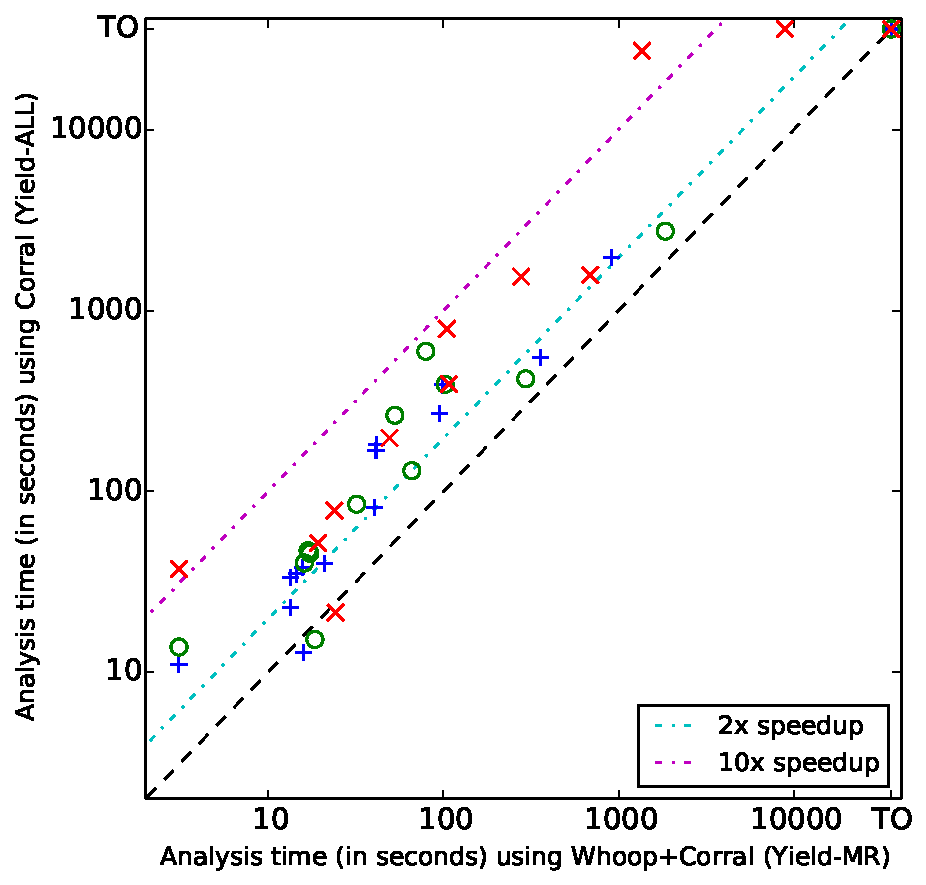
\includegraphics[width=.99\linewidth]{experiments/figures/yieldmr_vs_yieldall.pdf}
\caption{Scatter plot showing the runtime speedups that \corral achieves using \whoop with the \yieldmr instrumentation. The symbols $+$, $\circ$ and $\times$, represent a context-switch bound of 2, 5 and 9, respectively.}
\label{fig:plot}
\end{figure}

We performed experiments to validate the usefulness of the \whoop approach (Section~\ref{whoop}) and its combination with \corral (Section~\ref{corral}). We first present race-checking results from running \whoop and \corral on \sizeOfBenchmarks drivers taken from the 4.0 Linux kernel distribution.\footnote{\url{https://www.kernel.org}} We then evaluate the runtime performance and scalability of \corral and \whoop + \corral with different yield instrumentation granularities and context-switch bounds.
Our results demonstrate that \whoop can efficiently accelerate race-checking with \corral.

\noindent
\textbf{Experimental Setup}\xspace\xspace We performed all experiments on a 3.40GHz Intel Core i7-2600 CPU with 16GB RAM running Ubuntu Linux 12.04.5 LTS, LLVM 3.5, SMACK 1.5, Z3 4.3.2, Boogie rev. 4192 and \corral rev. 534.  \ADComment{Perhaps also state that Boogie runs inside Mono, and give the Mono version?}

\noindent
\textbf{Benchmarks}\xspace\xspace We evaluate our methodology against \sizeOfBenchmarks drivers taken from the 4.0 Linux kernel. We chose non-trivial drivers from several domains: block; char; ethernet; near field communication (nfc); universal serial bus (usb); and watchdog. We had to manually model the environment for these drivers, a process that required approximately two months of work.  \ADComment{Question from me: are block and char domains, in the same way that ethernet is a domain?}

\ADComment{At this point, is it absolutely clear what we do with \corral?  I.e., that we consider each entry point pair separately, and do not employ any abstraction to model additional threads?}

\noindent
\textbf{Race-Checking}\xspace\xspace Table~\ref{tab:stats} presents statistics for all our benchmarks: lines of code (LoC); number of entry point pairs (\#Pairs); number of SMACK memory regions (\#MRs); number of potentially racy pairs identified by \whoop (\#Racy Pairs); number of potentially racy memory regions reported by \whoop (\#Racy MRs); and number of races discovered by \corral using a context-switch bound of 2 (\#Races Found). We did not discover new races with larger context-switch bounds. This might mean that these drivers only have races that manifest with at least one or two context-switches, or that \corral hit its bounds before discovering a deeper race.

We can see that \whoop reports more races than \corral. This is expected, since \whoop employs an over-approximating shared state abstraction to conservatively model the effects of additional threads when analysing an entry point pair, and because lockset analysis is inherently imprecise; both factors can lead to false alarm race reports.  On the other hand, \corral is precise, but can miss races because only a limited number of context switches are considered.  Another issue with \corral is loop coverage due to unsound loop unrolling. To tackle this, we enable the built-in loop over-approximation described in~\cite{lal2014powering}. This can potentially lead \corral to report false positives, but we have not seen this in practice.  \ADComment{Would this be a good point to reiterate the fact that when we apply \corral to an entry point pair, we are just checking the specific pair of threads, and are not accounting for actions by other threads?}

Most of the races that \whoop and \corral discovered can be classified in two cases. The first case is accessing a global counter (or flag) from concurrent entry points, without a lock. This might be for performance, and indeed a lot of the races we found might be benign. Even benign races, though, lead to undefined behavior according to the C standard, and it is well known that undefined behaviors can lead to unexpected results when combined with aggressive compiler optimizations. The second case is an entry point accessing a field of an object (either global or passed as a parameter) without a lock. This can lead to a race if another entry point simultaneously accesses the same field of the same object.

As an example of the second case, we found the following race in the generic\_nvram char driver (see Figure~\ref{fig:data_race_example} for the source code): during the \texttt{llseek} entry point, the driver is accessing the file offset \texttt{file->f\_pos} without first acquiring a lock (\texttt{file} is passed as a parameter to \texttt{llseek}). This can lead to a race if the driver invokes \texttt{llseek} from another thread passing the same \texttt{file} object as a parameter. When we investigated another char driver that uses the same APIs, we saw that it was protecting the offset access in its \texttt{llseek} entry point with a mutex. This made us suspicious that the race we found in generic\_nvram could be real. We filed a bug report, but did not manage to get a response yet.

\noindent
\textbf{Granularity of Context-Switches}\xspace\xspace Table~\ref{tab:results} presents runtime results from using \whoop, \corral and \whoop + \corral to analyze our benchmarks. All reported times, in seconds, are averages over three runs. \ADComment{Can we say something about variance?  Perhaps ask Nathan what best to say?} \corral was given a time budget of 10 hours (T.O. denotes a tool timeout), and we considered context-switch bounds (csb) of 2, 5 and 9. By default, \corral instruments context-switches (i.e. \texttt{yield} statements) in \ADComment{instead of ``in'' can we say either ``before'' or ``after'' (not sure which is accurate)} all visible operations (denoted \yieldall). \whoop + \corral, instead, uses two different context-switch instrumentation granularities, \yieldcoarse and \yieldmr (see Section~\ref{whoop:bugfinding}), and also uses all the optimisations discussed in Section~\ref{whoop:optimizations}.

A higher context-switch bound results into deeper interleavings being explored and thus a larger sequentialized program. Intuitively, this means that we see even greater speedups using information from \whoop, when exploring deeper interleavings.

We can notice that \whoop is significantly faster than \corral. This is expected as \whoop achieves scalability using over-approximation and summarization techniques. This allows \whoop to perform especially well in complex drivers such as the r8169 ethernet driver: although \corral ... and timeouts with a csb of 9, \whoop manages to analyze the driver in 228.1 seconds. We believe that the reason behind this is that r8169 has many loops and uses deeply-nested recursion in some entry points, which \corral might not be able to handle efficiently.

%When running \corral on its own, it can potentially report a spurious race (that \whoop does not report), because \corral is not enhanced with domain-specific information that \whoop uses to discard spurious races. Using \whoop + \corral, though, will inherently discard spurious data races (assuming a precise environmental model).

%When \corral on its own tries to analyze the machzwd watchdog driver it explodes, because in some entry point pairs it attempts to analyze a large number of memory regions. For example for the entry point pair write vs init, it instruments interleavings at 26 different memory regions in a single invocation of \corral, which required approximately 1000 seconds to analyze. The same entry point pair is found race-free by \whoop. Using this information in \corral with the \yieldmr instrumentation, the pair takes less than a second to analyze. The \yieldcoarse instrumentation does not perform as well, because it works in the binary granularity of racy or non-racy entry points.


\section{Related Work}

Statically analyzing concurrent programs to detect races is a promising alternative to dynamic analyzers, which commonly face code coverage issues as they rely on a (controlled) scheduler for exploring execution paths~\cite{musuvathi2008finding}. Warlock~\cite{sterling1993warlock} and LockLint~\cite{oracle2010locklint} are notable examples of static race analyzers. However, both tools have limited applicability, as they heavily rely on user annotations. \textsc{Whoop}, on the other hand, does not require any source code modifications, and thus can be applied with minimal effort.

Most related to our work are the static lockset analyzers RELAY~\cite{voung2007relay} and Locksmith~\cite{pratikakis2006locksmith}. Both tools, though, have significant limitations. The authors of RELAY found 5022 warnings when analyzing the Linux kernel, with only 25 of them being true data races. To limit these false positives, RELAY employs post-analysis unsound filters, but these can also filter out true races. Although Locksmith successfully detected data races in several small Pthreads applications and 7 medium-sized Linux device drivers, it also reported a significant number of false positives. The authors also reported that Locksmith was unable to run on several large programs, showcasing its limited scalability. In contrast, \whoop is based on novel over-approximation techniques and uses modern SMT solvers to accelerate state-of-the-art concurrency bug-finders, such as \corral, for precise \emph{and} scalable analysis.

\section{Conclusions}

In this paper, we presented \whoop, a novel infrastructure for (i) analyzing the concurrent behavior of Linux drivers and (ii) accelerating a plugged-in bug-finder using information from our static data race analysis. In the heart of our approach, we combine static lock set analysis with sound sequentialization and automated theorem proving. Our lock set analysis enforces the locking discipline that two threads accessing the same shared resource must hold at least one common lock, and reports a potential data race if this discipline is violated.

Compared to traditional data race detection tools that typically attempt to explore as many thread interleavings as feasible, and thus face scalability issues in the presence of realistic concurrent programs, \textsc{Whoop} not only entirely avoids reasoning about thread interleavings, but also allows the reuse of existing successful sequential verification techniques. The main limitation of our approach is that it can potentially report many false positives, as we over-approximate the device driver shared state. To tackle this problem, we use the race-related information that \whoop generates to speed up \corral, a state-of-the-art precise bug-finder for concurrent programs.

% An example of a floating figure using the graphicx package.
% Note that \label must occur AFTER (or within) \caption.
% For figures, \caption should occur after the \includegraphics.
% Note that IEEEtran v1.7 and later has special internal code that
% is designed to preserve the operation of \label within \caption
% even when the captionsoff option is in effect. However, because
% of issues like this, it may be the safest practice to put all your
% \label just after \caption rather than within \caption{}.
%
% Reminder: the "draftcls" or "draftclsnofoot", not "draft", class
% option should be used if it is desired that the figures are to be
% displayed while in draft mode.
%
%\begin{figure}[!t]
%\centering
%\includegraphics[width=2.5in]{myfigure}
% where an .eps filename suffix will be assumed under latex, 
% and a .pdf suffix will be assumed for pdflatex; or what has been declared
% via \DeclareGraphicsExtensions.
%\caption{Simulation Results}
%\label{fig_sim}
%\end{figure}

% Note that IEEE typically puts floats only at the top, even when this
% results in a large percentage of a column being occupied by floats.


% An example of a double column floating figure using two subfigures.
% (The subfig.sty package must be loaded for this to work.)
% The subfigure \label commands are set within each subfloat command, the
% \label for the overall figure must come after \caption.
% \hfil must be used as a \section{?}
% separator to get equal spacing.
% The subfigure.sty package works much the same way, except \subfigure is
% used instead of \subfloat.
%
%\begin{figure*}[!t]
%\centerline{\subfloat[Case I]\includegraphics[width=2.5in]{subfigcase1}%
%\label{fig_first_case}}
%\hfil
%\subfloat[Case II]{\includegraphics[width=2.5in]{subfigcase2}%
%\label{fig_second_case}}}
%\caption{Simulation results}
%\label{fig_sim}
%\end{figure*}
%
% Note that often IEEE papers with subfigures do not employ subfigure
% captions (using the optional argument to \subfloat), but instead will
% reference/describe all of them (a), (b), etc., within the main caption.


% An example of a floating table. Note that, for IEEE style tables, the 
% \caption command should come BEFORE the table. Table text will default to
% \footnotesize as IEEE normally uses this smaller font for tables.
% The \label must come after \caption as always.
%
%\begin{table}[!t]
%% increase table row spacing, adjust to taste
%\renewcommand{\arraystretch}{1.3}
% if using array.sty, it might be a good idea to tweak the value of
% \extrarowheight as needed to properly center the text within the cells
%\caption{An Example of a Table}
%\label{table_example}
%\centering
%% Some packages, such as MDW tools, offer better commands for making tables
%% than the plain LaTeX2e tabular which is used here.
%\begin{tabular}{|c||c|}
%\hline
%One & Two\\
%\hline
%Three & Four\\
%\hline
%\end{tabular}
%\end{table}


% Note that IEEE does not put floats in the very first column - or typically
% anywhere on the first page for that matter. Also, in-text middle ("here")
% positioning is not used. Most IEEE journals/conferences use top floats
% exclusively. Note that, LaTeX2e, unlike IEEE journals/conferences, places
% footnotes above bottom floats. This can be corrected via the \fnbelowfloat
% command of the stfloats package.


% use section* for acknowledgement
\section*{Acknowledgments}
We would like to thank Akash Lal for his useful input and helping us with various \corral issues. Further, we would like to acknowledge Montgomery Carter for developing SMACK models for Linux locks, and Anton Burtsev, Charlie Jacobsen and the members of the Multicore Programming Group of Imperial College London for discussions and feedback in various stages of this work. This work is part of the research project ``Automatic Synthesis of High-Assurance Device Drivers'' and is generously funded by a gift from Intel Corporation.

% trigger a \newpage just before the given reference
% number - used to balance the columns on the last page
% adjust value as needed - may need to be readjusted if
% the document is modified later
%\IEEEtriggeratref{8}
% The "triggered" command can be changed if desired:
%\IEEEtriggercmd{\enlargethispage{-5in}}

% references section

% can use a bibliography generated by BibTeX as a .bbl file
% BibTeX documentation can be easily obtained at:
% http://www.ctan.org/tex-archive/biblio/bibtex/contrib/doc/
% The IEEEtran BibTeX style support page is at:
% http://www.michaelshell.org/tex/ieeetran/bibtex/
\bibliographystyle{IEEEtran}
% argument is your BibTeX string definitions and bibliography database(s)
\bibliography{references}
%
% <OR> manually copy in the resultant .bbl file
% set second argument of \begin to the number of references
% (used to reserve space for the reference number labels box)
%\begin{thebibliography}{1}

%\bibitem{IEEEhowto:kopka}
%H.~Kopka and P.~W. Daly, \emph{A Guide to \LaTeX}, 3rd~ed.\hskip 1em plus
 % 0.5em minus 0.4em\relax Harlow, England: Addison-Wesley, 1999.

%\end{thebibliography}




% that's all folks
\end{document}


